\subsubsection{概要}
むぎまるチームは1章で述べた目標のために, 
価値反復ROSパッケージと,ともに使用するパッケージを開発した.
自己位置推定には,昨年のきなこチームの使用したシステムをそのまま用いている.
パッケージであるemcl2\_ros2\cite{emcl2_ros2}を使用した. 
%@@@↑これだと目標のために
%@@@(人の作った)emcl2_ros2を使ってるという感じになってよくないです. 
%@@@emcl2_ros2は自分たちでメンテナンスしてるんですから, 自分たちのものだと明記を. 

\subsubsection{システム構成}
ロボットに搭載した計算機, センサ, アクチュエータの接続の関係及び
計算機で実行するROS 2ノードの概要を表したものを
図\ref{fig:mugimaru_system}に示す. 

Raspberry Piには, 車体制御のために, IMUとエンコーダ, 車輪駆動用のモータを接続した. 
実行するノードとしては, IMU用のROS 2ドライバノード(rt\_usb\_9axisimu\_driver)と, 
オドメトリの出力とモータの制御を実施するノード(raspimouse)がある. 
後者のノードでは, エンコーダの値と
前者のノードで配信されたIMUの情報からロボットのオドメトリを計算し, 
トピックとして配信する. 
モータの制御は, 外部のノードからトピックとして受信した
ロボットの速度指令をもとに実行する. 

miniPCはRaspberry Piから
オドメトリのトピックを受け入れる. 
また, 3D LiDARが物理的に接続される. 
実行されるノードとしては, 3D LiDARに関係するもの: 
\begin{itemize}
	\item livox\_lidar\_publisher: Livox用のROS 2ドライバノード
	\item pointcloud\_to\_laserscan: 3D LiDARのスキャンデータを2次元に圧縮してトピックとして配信するノード
\end{itemize}
と, 自己位置推定とナビゲーションに関係するもの: 
\begin{itemize}
	\item emcl2\_ros2: 自己位置推定ノード(図中では「emcl2」と表記)
	\item 価値反復
\end{itemize}
がある. 

走行する環境の地図は,GLIMで作成したものを
高さ方向で切り出したものを使用した.
切り出しにはpointcloud2pgm\_slicerを用いた.



%書き換える
\begin{figure}[h]
  \begin{center}
    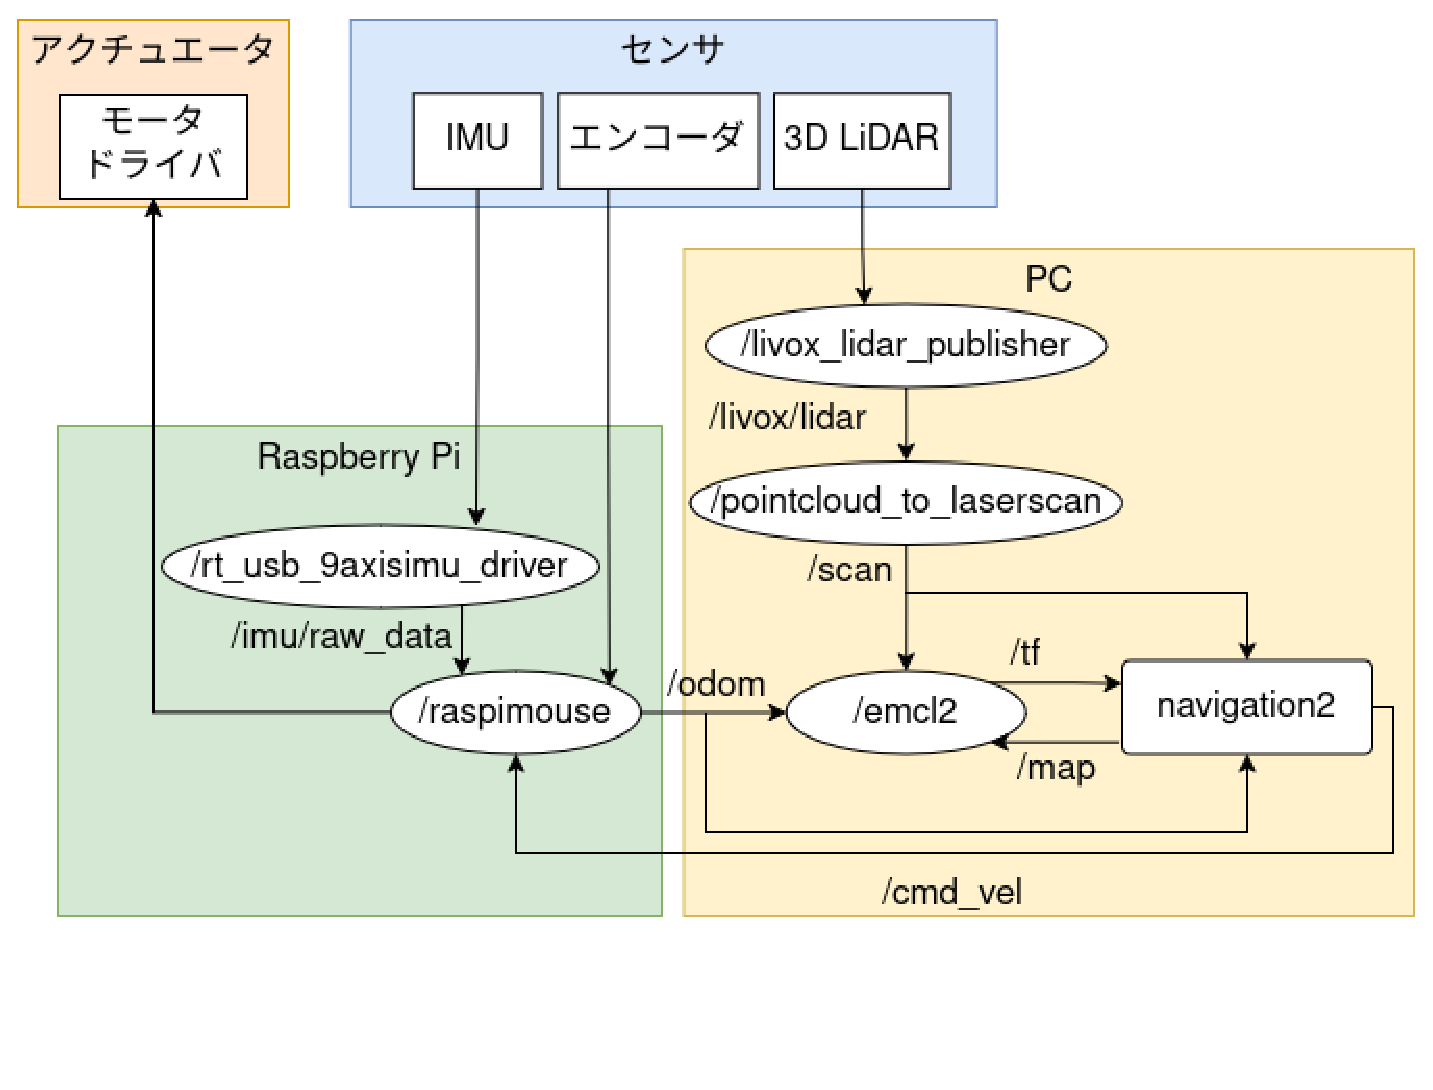
\includegraphics[width=1.0\linewidth]{figs/mugimaru_system_2024.eps}
    \caption{むぎまるチームのシステム構成}
    \label{fig:mugimaru_system}
  \end{center}
\end{figure}

